\let\negmedspace\undefined
\let\negthickspace\undefined
\documentclass[journal,12pt,onecolumn]{IEEEtran}
\usepackage{cite}
\usepackage{amsmath,amssymb,amsfonts,amsthm}
\usepackage{algorithmic}
\usepackage{graphicx}
\usepackage{textcomp}
\usepackage{xcolor}
\usepackage{txfonts}
\usepackage{listings}
\usepackage{enumitem}
\usepackage{mathtools}
\usepackage{gensymb}
\usepackage[breaklinks=true]{hyperref}
\usepackage{tkz-euclide} % loads  TikZ and tkz-base
\usepackage{listings}
\usepackage[siunitx]{circuitikz}[american voltages]
\usetikzlibrary{decorations.markings}

\newtheorem{theorem}{Theorem}[section]
\newtheorem{problem}{Problem}
\newtheorem{proposition}{Proposition}[section]
\newtheorem{lemma}{Lemma}[section]
\newtheorem{corollary}[theorem]{Corollary}
\newtheorem{example}{Example}[section]
\newtheorem{definition}[problem]{Definition}
%\newtheorem{thm}{Theorem}[section] 
%\newtheorem{defn}[thm]{Definition}
%\newtheorem{algorithm}{Algorithm}[section]
%\newtheorem{cor}{Corollary}
\newcommand{\BEQA}{\begin{eqnarray}}
\newcommand{\EEQA}{\end{eqnarray}}
\newcommand{\system}[1]{\stackrel{#1}{\rightarrow}}
\newcommand{\define}{\stackrel{\triangle}{=}}
\theoremstyle{remark}
\newtheorem{rem}{Remark}
%\bibliographystyle{ieeetr}
\begin{document}
%
\providecommand{\pr}[1]{\ensuremath{\Pr\left(#1\right)}}
\providecommand{\prt}[2]{\ensuremath{p_{#1}^{\left(#2\right)} }}        % own macro for this question
\providecommand{\qfunc}[1]{\ensuremath{Q\left(#1\right)}}
\providecommand{\sbrak}[1]{\ensuremath{{}\left[#1\right]}}
\providecommand{\lsbrak}[1]{\ensuremath{{}\left[#1\right.}}
\providecommand{\rsbrak}[1]{\ensuremath{{}\left.#1\right]}}
\providecommand{\brak}[1]{\ensuremath{\left(#1\right)}}
\providecommand{\lbrak}[1]{\ensuremath{\left(#1\right.}}
\providecommand{\rbrak}[1]{\ensuremath{\left.#1\right)}}
\providecommand{\cbrak}[1]{\ensuremath{\left\{#1\right\}}}
\providecommand{\lcbrak}[1]{\ensuremath{\left\{#1\right.}}
\providecommand{\rcbrak}[1]{\ensuremath{\left.#1\right\}}}
\newcommand{\sgn}{\mathop{\mathrm{sgn}}}
\providecommand{\abs}[1]{\left\vert#1\right\vert}
\providecommand{\res}[1]{\Res\displaylimits_{#1}} 
\providecommand{\norm}[1]{\left\lVert#1\right\rVert}
%\providecommand{\norm}[1]{\lVert#1\rVert}
\providecommand{\mtx}[1]{\mathbf{#1}}
\providecommand{\mean}[1]{E\left[ #1 \right]}
\providecommand{\cond}[2]{#1\middle|#2}
\providecommand{\fourier}{\overset{\mathcal{F}}{ \rightleftharpoons}}
\newenvironment{amatrix}[1]{%
  \left(\begin{array}{@{}*{#1}{c}|c@{}}
}{%
  \end{array}\right)
}
%\providecommand{\hilbert}{\overset{\mathcal{H}}{ \rightleftharpoons}}
%\providecommand{\system}{\overset{\mathcal{H}}{ \longleftrightarrow}}
	%\newcommand{\solution}[2]{\textbf{Solution:}{#1}}
\newcommand{\solution}{\noindent \textbf{Solution: }}
\newcommand{\cosec}{\,\text{cosec}\,}
\providecommand{\dec}[2]{\ensuremath{\overset{#1}{\underset{#2}{\gtrless}}}}
\newcommand{\myvec}[1]{\ensuremath{\begin{pmatrix}#1\end{pmatrix}}}
\newcommand{\mydet}[1]{\ensuremath{\begin{vmatrix}#1\end{vmatrix}}}
\newcommand{\myaugvec}[2]{\ensuremath{\begin{amatrix}{#1}#2\end{amatrix}}}
\providecommand{\rank}{\text{rank}}
\providecommand{\pr}[1]{\ensuremath{\Pr\left(#1\right)}}
\providecommand{\qfunc}[1]{\ensuremath{Q\left(#1\right)}}
	\newcommand*{\permcomb}[4][0mu]{{{}^{#3}\mkern#1#2_{#4}}}
\newcommand*{\perm}[1][-3mu]{\permcomb[#1]{P}}
\newcommand*{\comb}[1][-1mu]{\permcomb[#1]{C}}
\providecommand{\qfunc}[1]{\ensuremath{Q\left(#1\right)}}
\providecommand{\gauss}[2]{\mathcal{N}\ensuremath{\left(#1,#2\right)}}
\providecommand{\diff}[2]{\ensuremath{\frac{d{#1}}{d{#2}}}}
\providecommand{\myceil}[1]{\left \lceil #1 \right \rceil }
\newcommand\figref{Fig.~\ref}
\newcommand\tabref{Table~\ref}
\newcommand{\sinc}{\,\text{sinc}\,}
\newcommand{\rect}{\,\text{rect}\,}
%%
%	%\newcommand{\solution}[2]{\textbf{Solution:}{#1}}
%\newcommand{\solution}{\noindent \textbf{Solution: }}
%\newcommand{\cosec}{\,\text{cosec}\,}
%\numberwithin{equation}{section}
%\numberwithin{equation}{subsection}
%\numberwithin{problem}{section}
%\numberwithin{definition}{section}
%\makeatletter
%\@addtoreset{figure}{problem}
%\makeatother

%\let\StandardTheFigure\thefigure
\let\vec\mathbf


\bibliographystyle{IEEEtran}
\title{GATE-EC-51}
\author{EE23BTECH11059- Tejas Mehtre$^{*}$% <-this % stops a space
}
\maketitle




\bigskip

\renewcommand{\thefigure}{\theenumi}
\renewcommand{\thetable}{\theenumi}
%\renewcommand{\theequation}{\theenumi}
Consider an FM broadcast that employs the pre-emphasis filter with frequency response \\
    \begin{align*}
        H_{pe}\brak{\omega}= 1+ \frac{j\omega}{\omega _0},
    \end{align*}
    where $\omega_0=10^4$ rad/sec. \\
    For the network shown in the figure to act as a corresponding de-emphasis filter, the
appropriate pair(s) of (R,C) values is/are 
\underline{\hspace{1in}} \\ \\
\begin{center}
    \begin{circuitikz}
		\draw
		(0,0)  to[resistor,*-,l=$R$] (4,0)
		to[capacitor,l=$C$] (4,-4) to (7,-4)
		(4,0) -- (7,0)
		(4,-4) to[short,-*] (0,-4);
		\node[below left] at (0,0){$+$};
		\node[above left] at (0,-4){$-$};
		\node[below right] at (7,0){$+$};
		\node[above right] at (7,-4){$-$};
		\draw [<->] (0,-0.3) -- (0,-3.7);
		\node[left] at (0,-2){input};
		\draw [<->] (7,-0.3) -- (7,-3.7);
		\node[right] at (7,-2){output};
	\end{circuitikz}
\end{center}
\begin{enumerate}
    \item[A.] $R=1k\ohm$, $C=0.1\micro F$
    \item[B.] $R=2k\ohm$, $C=1\micro F$
    \item[C.] $R=1k\ohm$, $C=2\micro F$
    \item[D.] $R=2k\ohm$, $C=0.5\micro F$
\end{enumerate}
  \solution
    \begin{table}[!ht]
    \centering
        \begin{tabular}[12pt]{ |c| c|c|}
    \hline
    \textbf{Parameter} & \textbf{Description} & \textbf{Value}\\ 
    \hline
    $y^{''} -  4y^{'} -12y = 3e^{5x}$ & Differential equation & none\\
    \hline
    $y\brak{x}$ &Solution of  differential equation & $y(0)=\frac{18}{7}$\\
    \hline
    $y^{'}\brak{x}$ & First order derivative of solution of differential equation & $y^{'}\brak{0}=\frac{-1}{7}$\\
    \hline
     \end{tabular} 

    \caption{input parameters}
    \label{}
\end{table}
\\
    Taking KVL around the loop,
    \begin{align}
        -V_i\brak{t} + i\brak{t}R + V_0\brak{t}=0 
    \end{align}
    \begin{align}
        \mathcal{L}\brak{f'\brak{t}} &\xleftrightarrow{\mathcal{L}} sF\brak{s}-f\brak{0} \label{q:2022/EC/51/1} \\
        i\brak{t}&= C\frac{dV_0\brak{t}}{dt} \label{eq:2022/EC/51/2}
    \end{align}
    Using \eqref{q:2022/EC/51/1} and \eqref{eq:2022/EC/51/2},
    \begin{align}
        \mathcal{L}\brak{ -V_i\brak{t} + RC\frac{dV_0\brak{t}}{dt} + V_0\brak{t}}&=\mathcal{L}\brak{0} \\
        V_0\brak{s}\brak{1+j\omega RC}&= V_i\brak{s} \\
         H\brak{j\omega}=\frac{V_o\brak{j\omega}}{V_i\brak{j\omega}} &= \frac{1}{1+j\omega RC}
    \end{align}
%Transfer function of the above $RC$ circuit will be
%\begin{align}
 %   H\brak{j\omega}=\frac{V_o\brak{j\omega}}{V_i\brak{j\omega}}= \frac{1}{1+j\omega RC}
%\end{align}
The given $RC$ circuit to act as de-emphasis filter
\begin{align}
    \abs{H\brak{j\omega}}&= \frac{1}{\abs{H_{pre}\brak{\omega}}} \\
    \frac{1}{\sqrt{1+\brak{\omega RC}^2}}&= \frac{1}{\sqrt{1+\brak{\frac{\omega}{\omega_0}}^2}} \\
    \omega_0&= \frac{1}{RC} \\
    \omega_0&=10^4 rad/sec
\end{align}
Thus $\omega_0=10^4$ rad/sec only possible if we choose $R=1k\ohm$ and $C=0.1\micro F$ from options. Hence, the correct option is (B).
\begin{figure}[ht]
        \centering
        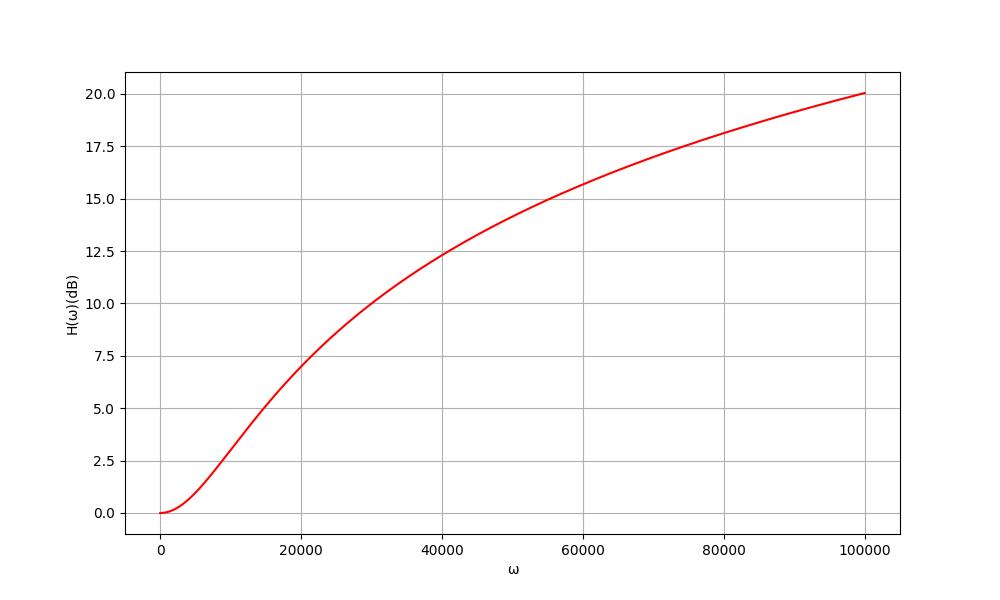
\includegraphics[width=\columnwidth]{figs/plot.png}
        \caption{Frequency response of a pre-emphasis filter.}
    \end{figure}
\end{document}
\end{document}
